\documentclass[tikz,border=2mm]{standalone}
\usepackage{amsmath,amssymb}
\usepackage{xcolor}
\usepackage{pifont}
\usetikzlibrary{positioning,arrows.meta,shapes.geometric,shadows.blur,decorations.pathreplacing,calc,fit,backgrounds}

\definecolor{jbrand}{RGB}{15,58,102}
\definecolor{jbrandlight}{RGB}{232,240,247}
\definecolor{jbrandline}{RGB}{184,206,224}
\definecolor{jgrey}{RGB}{90,90,90}
\definecolor{jamber}{RGB}{176,98,10}
\definecolor{jamberlight}{RGB}{250,240,224}

\begin{document}
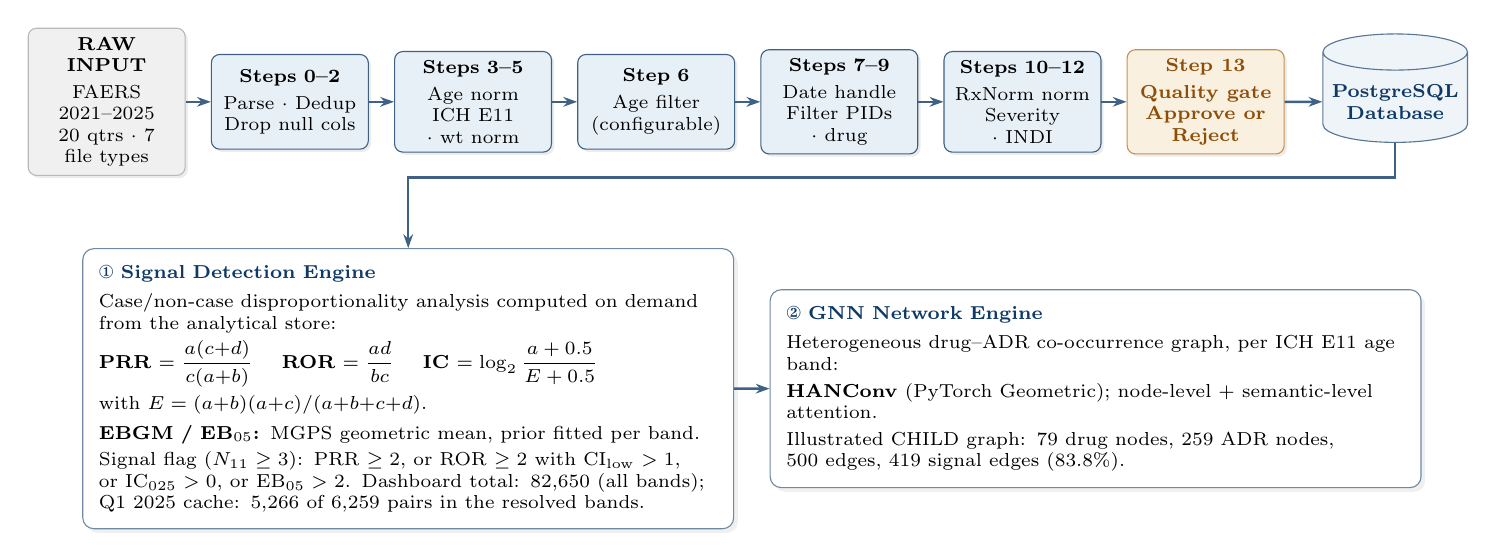
\begin{tikzpicture}[
  scale=0.97, every node/.append style={scale=0.97},
  font=\scriptsize,
  pipebox/.style={rectangle,rounded corners=3pt,draw=jbrand!80,fill=jbrandlight,
    minimum width=1.92cm,minimum height=1.24cm,align=center,text width=1.82cm,
    drop shadow={shadow xshift=1pt,shadow yshift=-1pt,opacity=0.15}},
  rawbox/.style={pipebox,fill=gray!12,draw=gray!55},
  gatebox/.style={pipebox,fill=jamberlight,draw=jamber!70,font=\scriptsize\bfseries,text=jamber!80!black},
  dbcyl/.style={cylinder,shape border rotate=90,draw=jbrand!70,fill=jbrandlight!70,
    aspect=0.25,minimum width=1.78cm,minimum height=1.42cm,align=center,font=\scriptsize\bfseries\color{jbrand}},
  engine/.style={rectangle,rounded corners=4pt,draw=jbrand!60,fill=white,inner sep=6pt,align=left,
    drop shadow={shadow xshift=1.5pt,shadow yshift=-1.5pt,opacity=0.12}},
  arr/.style={-{Stealth[length=5pt,width=3.5pt]},line width=0.9pt,color=jbrand!80},
]
\node[rawbox] (RAW) at (0,0) {\textbf{RAW INPUT}\\[2pt]FAERS 2021--2025\\20 qtrs $\cdot$ 7 file types};
\node[pipebox,right=0.32cm of RAW] (S02) {\textbf{Steps 0--2}\\[2pt]Parse $\cdot$ Dedup\\Drop null cols};
\node[pipebox,right=0.32cm of S02] (S35) {\textbf{Steps 3--5}\\[2pt]Age norm\\ICH E11 $\cdot$ wt norm};
\node[pipebox,right=0.32cm of S35] (S6) {\textbf{Step 6}\\[2pt]Age filter\\(configurable)};
\node[pipebox,right=0.32cm of S6] (S79) {\textbf{Steps 7--9}\\[2pt]Date handle\\Filter PIDs $\cdot$ drug};
\node[pipebox,right=0.32cm of S79] (S1012) {\textbf{Steps 10--12}\\[2pt]RxNorm norm\\Severity $\cdot$ INDI};
\node[gatebox,right=0.32cm of S1012] (S13) {\textbf{Step 13}\\[2pt]Quality gate\\Approve or\\Reject};
\node[dbcyl,right=0.48cm of S13] (DB) {PostgreSQL\\Database};
\draw[arr](RAW)--(S02); \draw[arr](S02)--(S35); \draw[arr](S35)--(S6);
\draw[arr](S6)--(S79); \draw[arr](S79)--(S1012); \draw[arr](S1012)--(S13); \draw[arr](S13)--(DB);

%% Engine panels — self-contained: no \ref or \cite, so the exported figure
%% carries no unresolved cross-references (PLOS figures are standalone files).
\node[engine,text width=8.1cm,below=1.25cm of S02.south,xshift=1.55cm] (SIG) {%
  {\color{jbrand}\textbf{\ding{172} Signal Detection Engine}}\\[3pt]
  Case/non-case disproportionality analysis computed on demand from the analytical store:\\[2pt]
  \textbf{PRR} $=\dfrac{a(c{+}d)}{c(a{+}b)}$ \quad
  \textbf{ROR} $=\dfrac{ad}{bc}$ \quad
  \textbf{IC} $=\log_2\dfrac{a+0.5}{E+0.5}$\\[2pt]with $E=(a{+}b)(a{+}c)/(a{+}b{+}c{+}d)$.\\[3pt]
  \textbf{EBGM / EB$_{05}$:} MGPS geometric mean, prior fitted per band.\\[2pt]
  Signal flag ($N_{11}\geq3$): PRR $\geq2$, or ROR $\geq2$ with CI$_{\mathrm{low}}>1$,\\
  or IC$_{025}>0$, or EB$_{05}>2$. Dashboard total: 82{,}650 (all bands);\\
  Q1 2025 cache: 5{,}266 of 6{,}259 pairs in the resolved bands.};
\node[engine,text width=8.1cm,right=0.45cm of SIG] (GNN) {%
  {\color{jbrand}\textbf{\ding{173} GNN Network Engine}}\\[3pt]
  Heterogeneous drug--ADR co-occurrence graph, per ICH~E11 age band:\\[2pt]
  \textbf{HANConv} (PyTorch Geometric); node-level $+$ semantic-level attention.\\[2pt]
  Illustrated CHILD graph: 79 drug nodes, 259 ADR nodes,\\
  500 edges, 419 signal edges (83.8\%).};
\draw[arr](DB.south)--++(0,-0.45)-|(SIG.north);
\draw[arr](SIG.east)--(GNN.west);
\end{tikzpicture}
\end{document}
